\begin{frame}[label=background]{Structure Background}
    \frametitle{Structure}
    \begin{itemize}
        \item Research Questions
        \item {\color{tud grapefruit}Mathematical Background}
        \item Related Work
        \item Preliminary Results
        \item Outlook
    \end{itemize}
\end{frame}

\footerinfootnotestrue
\begin{frame}[label=background,fragile]{Background: CG method}
    \frametitle{Mathematical Background}
    \framesubtitle{Conjugate gradient method}
    \begin{algorithm}[H]
        \begin{algorithmic}
            \State $\mathbf{r}_0 = \mathbf{b} - A\mathbf{u}_0$, $\mathbf{p}_0 = \mathbf{r}_0$, $\beta_0 = 0$
            \For{$j = 0, 1, 2, \dots, m$}
            \State $\alpha_j = (\mathbf{r}_j, \mathbf{r}_j) / (A \mathbf{p}_j, \mathbf{p}_j)$
            \State $\mathbf{u}_{j+1} = \mathbf{u}_j + \alpha_j \mathbf{p}_j$
            \State $\mathbf{r}_{j+1} = \mathbf{r}_j - \alpha_j A \mathbf{p}_j$
            \State $\beta_j = (\mathbf{r}_{j+1}, \mathbf{r}_{j+1}) / (\mathbf{r}_j, \mathbf{r}_j)$
            \State $\mathbf{p}_{j+1} = \mathbf{r}_{j+1} + \beta_j \mathbf{p}_j$
            \EndFor
        \end{algorithmic}
        \caption{Conjugate Gradient Method \cite{iter_method_saad}}
    \end{algorithm}
\end{frame}

\footerinfootnotesfalse
\begin{frame}[label=background,fragile]{Background: CG explained}
    \frametitle{Mathematical Background}
    \framesubtitle{Conjugate gradient method}
    \begin{columns}[T,onlytextwidth]
        \begin{column}{.5\textwidth}
            \begin{itemize}
                \item<+-> Iterative, projection method onto a Krylov subspace $\mathcal{K}_m(A_0, \mathbf{r}_0)$ given by
                \begin{equation*}
                     \text{span}\{\mathbf{r}_0, A\mathbf{r}_0, A^2\mathbf{r}_0, \dots, A^{m-1}\mathbf{r}_0\}
                \end{equation*}
                \item<+-> Approximate solution can be expressed as
                \begin{equation*}
                    \mathbf{u}_m = \mathbf{u}_0 + \sum_{i=0}^{m-1} c_i A^i \mathbf{r}_0 = \mathbf{u}_0 + \alert<3>{q_{m-1}}(A)\mathbf{r}_0
                \end{equation*}
                \item<4> Minimize residual polynomial on eigenvalues of $A$
            \end{itemize}
        \end{column}
        \begin{column}{.5\textwidth}
            \only<3-4>{%
                \begin{figure}
                    \centering
                    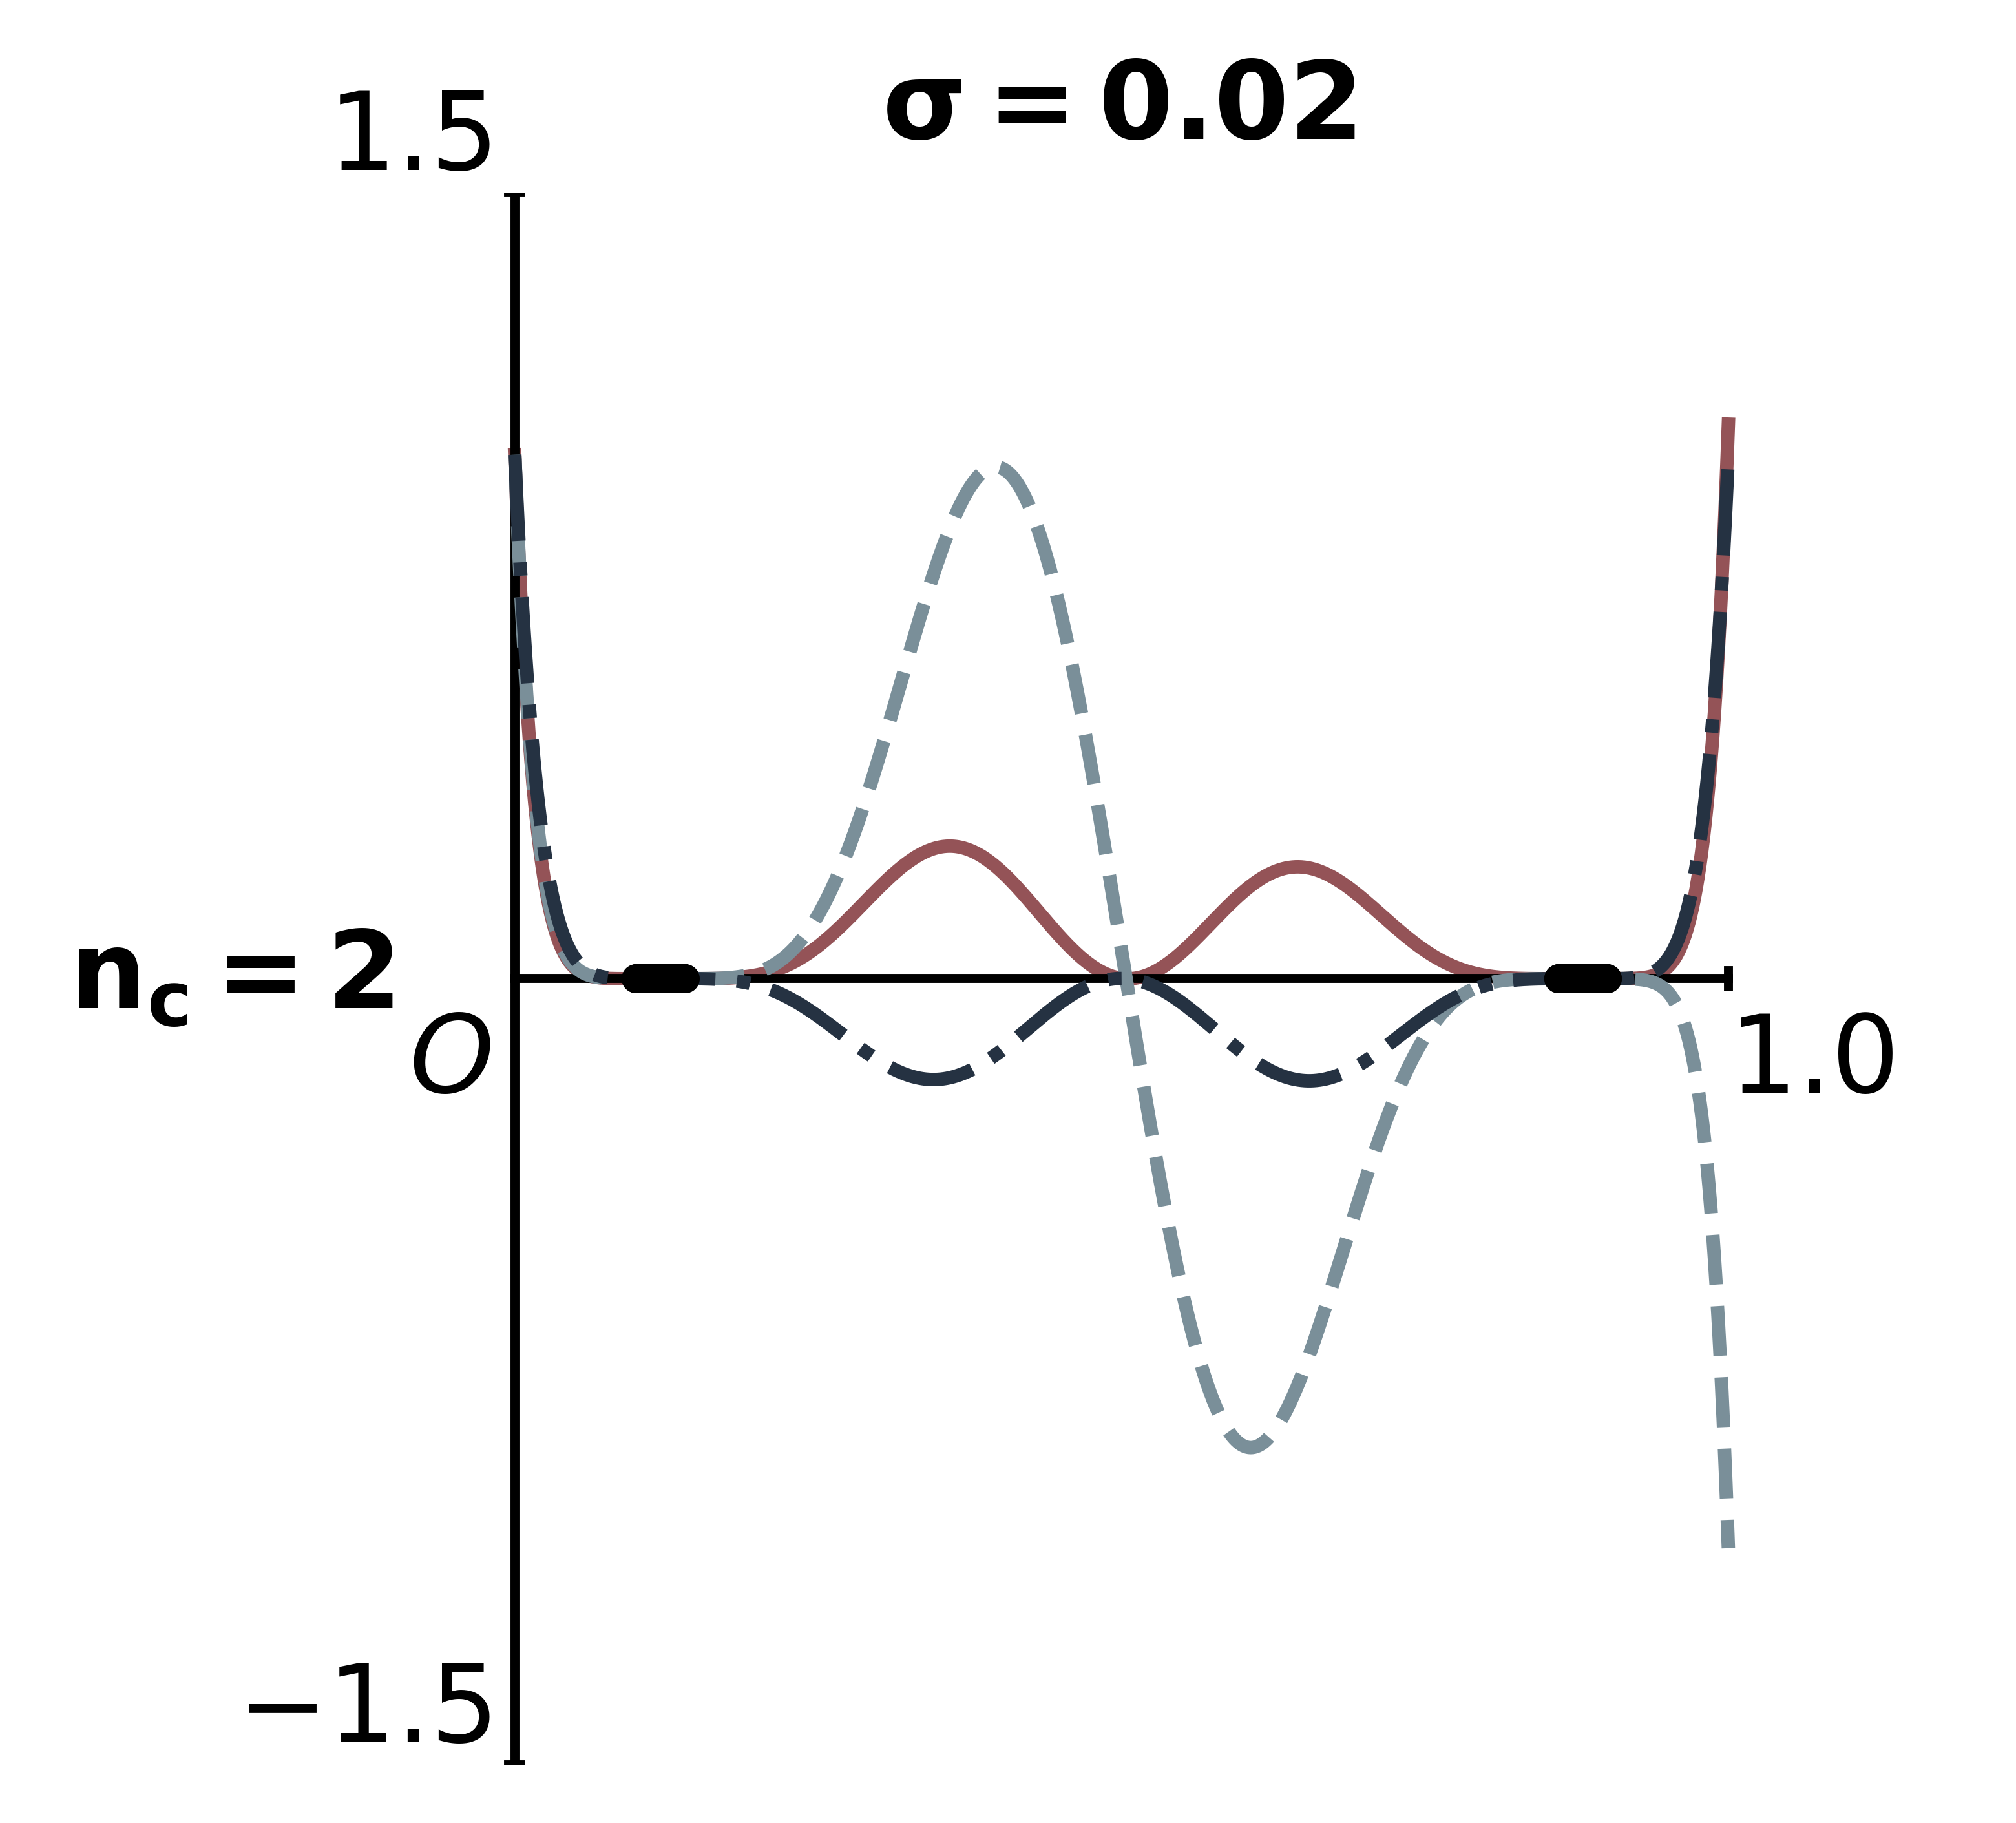
\includegraphics[width=0.8\textwidth]{two_cluster_respoly.png}
                    \caption{Residual polynomial $r_m(\lambda) = 1 - \lambda \alert<3>{q_{m-1}}(\lambda)$}
                \end{figure}
            }
        \end{column}
    \end{columns}
\end{frame}

\begin{frame}[label=background,fragile]{CG convergence}
    \frametitle{Mathematical Background}
    \framesubtitle{Conjugate gradient method}
    \begin{itemize}
        \item<1-> Classical (condition number) convergence bound:
        \begin{theorem}
            The error of the $m^{\text{th}}$ iterate of the CG algorithm is bounded by
            \begin{equation*}
            ||\mathbf{e}_m|| \leq 2 \left(\frac{\sqrt{\kappa}-1}{\sqrt{\kappa} + 1}\right)^m ||\mathbf{e}_0||_A,
            \end{equation*}
            where $\kappa = \lambda_{\text{max}}/\lambda_{\text{min}}$ is the condition number of (symmetric matrix) $A$.
        \end{theorem}
        \item<2-> Only sharp for \alert<2>{uniform} eigenvalue distributions!
        \begin{equation*}
            ||\mathbf{e}_m||_A \leq \min_{r \in \mathcal{P}_{m-1}, r(0) = 1} \max_{\lambda \in [\lambda_{\text{min}}, \lambda_{\text{max}}]} |r(\lambda)| ||\mathbf{e}_0||_A \overset{\alert<2>{\text{uniform } \sigma(A)}}{=} \frac{\|\mathbf{e}_0\|}{C_m\left(\frac{\kappa + 1}{\kappa - 1}\right)}
        \end{equation*}
    \end{itemize}
\end{frame}

\begin{frame}[label=background,fragile]{CG spectra}
    \frametitle{Mathematical Background}
    \framesubtitle{Conjugate gradient method}
    Setting $\lambda_{\text{min}} = 0.1$ and $\lambda_{\text{max}} = 0.9$ gives $m_{\text{classical}} = 26$. \only<1>{\textcolor{tud grapefruit}{Worst case}}\only<2>{\textcolor{tud green}{Best case}} distribution:
    \only<1>{%
        \begin{figure}
            \centering
            \includegraphics[width=0.7\textwidth]{cg_convergence_extreme_spectra_cluster1.pdf}
            \caption{CG convergence for uniform spectrum.}
        \end{figure}
    }
    \only<2>{%
        \begin{figure}
            \centering
            \includegraphics[width=0.7\textwidth]{cg_convergence_extreme_spectra_cluster0.pdf}
            \caption{CG convergence for spectrum with two distinct eigenvalues.}
        \end{figure}
    }
\end{frame}

\footerinfootnotestrue
\begin{frame}[label=background,fragile]{Background: Schwarz}
    \frametitle{Mathematical Background}
    \framesubtitle{Schwarz preconditioners}
    \begin{columns}[T,onlytextwidth]
        \begin{column}{.5\textwidth}
            \begin{itemize}
                \item<1-> Derived from the Alternating Schwarz method\cite{schwarz_methods_Dolean_2015}
                \item<2-> Convergence rate depends on the overlap $\alert<2>{\delta}$ and the wave number of eigenmodes $\alert<3>{k}$
                \item<4-> As a preconditioner $M_{\text{ASM}} = \sum_{i=1}^{N_{\text{sub}}} R_i^T A_i^{-1} R_i$
                \item<5-> Need a coarse space $\alert<6>{R_0}$ to counter slowly converging modes
            \end{itemize}
        \end{column}
        \begin{column}{.49\textwidth}
            \only<1>{%
                \begin{figure}[H]
                    \begin{tikzpicture}[scale=1.5]
    
% Disk (left) % Smaller square (right): edges
\draw[chapter, thick] (-2,0) circle (1.2);
\draw[chapter, thick] (-1.8,-1.0) rectangle (0.2,1.0);

% Square (right) % Larger disk (left): fill
\fill[chapter!20] (-2,0) circle (1.2);
\fill[chapter!20] (-1.8,-1.0) rectangle (0.2,1.0);

% Overlapping region
\begin{scope}
  \clip (-2,0) circle (1.2);
  \fill[black!30, opacity=0.4] (-1.8,-1.0) rectangle (0.2,1.0);
\end{scope}

% Transparent edge in overlap (disk)
\begin{scope}
  \clip (-1.8,-1.0) rectangle (0.2,1.0);
  \draw[chapter, thick, opacity=0.3] (-2,0) circle (1.2);
\end{scope}

% Transparent edge in overlap (square)
\begin{scope}
  \clip (-2,0) circle (1.2);
  \draw[chapter, thick, opacity=0.3] (-1.8,-1.0) rectangle (0.2,1.0);
\end{scope}

% Labels
\node at (-3,1.2) {\Large $\Omega_1$};
\node at (0.3,1.2) {\Large $\Omega_2$};
\node at (-1.3,0.1) {\large $\Omega_1 \cap \Omega_2$};
    
\end{tikzpicture}
                    \caption{Domain decomposition with overlapping subdomains.}
                \end{figure}
            }
            \only<2-3>{%
                \begin{exampleblock}{2D Alternating Schwarz Example}
                    Let $\Omega_1 = (-\infty, \delta)\times \mathbb{R}$, $\Omega_2 = (\delta, \infty)\times \mathbb{R}$
                    \begin{align*}
                        -(\eta - \Delta) u & = f \text{ in } \mathbb{R}^2, \\
                        u                  & \text{ bounded at infinity}.
                    \end{align*}
                    Then the convergence rate is given by
                    \begin{equation*}
                        \rho_{\text{2D}}(k;\eta,\delta) = e^{-\alert<2>{\delta}\sqrt{\eta + \alert<3>k^2}}
                    \end{equation*}
                \end{exampleblock} 
            }
            \only<4-5>{%
                \begin{figure}[H]
                    \centering
                    % \begin{tikzpicture}[scale=1.2]

% % Draw the global square domain
% \draw[thick] (0,0) rectangle (3,3);
% % \node at (3.3,3.3) {$\Omega$};

% % Draw vertical and horizontal grid lines
% \foreach \x in {1,2} {
%     \draw[thick] (\x,0) -- (\x,3);
%     \draw[thick] (0,\x) -- (3,\x);
% }

% % Label subdomains
% \foreach \i in {0,1,2} {
%     \foreach \j in {0,1,2} {
%         \pgfmathtruncatemacro{\idx}{\i*3 + \j + 1}
%         \node at (0.5 + \j, 2.5 - \i) {$\Omega_{\idx}$};
%     }
% }

% \end{tikzpicture}
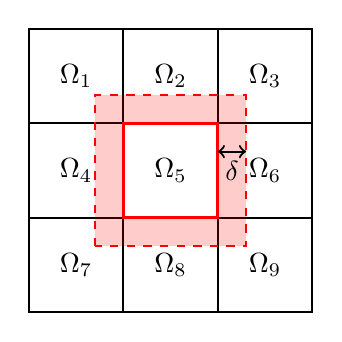
\begin{tikzpicture}[scale=1.2]

    % Draw the global square domain
    \draw[thick] (0,0) rectangle (3,3);
    
    % Draw vertical and horizontal grid lines
    \foreach \x in {1,2} {
        \draw[thick] (\x,0) -- (\x,3);
        \draw[thick] (0,\x) -- (3,\x);
    }
    
    % Label subdomains
    \foreach \i in {0,1,2} {
        \foreach \j in {0,1,2} {
            \pgfmathtruncatemacro{\idx}{\i*3 + \j + 1}
            \node at (0.5 + \j, 2.5 - \i) {$\Omega_{\idx}$};
        }
    }
    
    % Fill overlapping region around Omega_5
    \begin{scope}
        \clip (0.7,0.7) rectangle (2.3,2.3);
        \fill[red, opacity=0.2] (0.7,0.7) rectangle (2.3,2.3);
        \fill[white] (1,1) rectangle (2,2);
    \end{scope}
    
    % Redraw Omega_5 label on top
    \node at (1.5,1.5) {$\Omega_{5}$};

    % Draw dashed border for total overlap area
    \draw[dashed, thick, red] (0.7,0.7) rectangle (2.3,2.3);
    
    % Draw original Omega_5 boundary
    \draw[very thick, red] (1,1) rectangle (2,2);
    
    % Label delta
    \draw[<->, thick] (2,1.7) -- (2.3,1.7);
    \node[below] at (2.15,1.7) {$\delta$};
    
\end{tikzpicture}
    
                    \caption{Domain decomposition with $N_{\text{sub}}$ subdomains.}
                \end{figure}
            }
            \only<6>{%
            \begin{block}{2-level Additive Schwarz Preconditioner}
                \begin{equation*}
                    M_{\text{ASM,2}} = \alert<6>{R_0}^T A_0^{-1} \alert<6>{R_0} + M_{\text{ASM}}
                \end{equation*}
            \end{block} 
            }
        \end{column}
    \end{columns}
\end{frame}